\documentclass{book}
%\usepackage[a4paper]{geometry}
\usepackage{graphicx}
\usepackage{color}
\usepackage{url}
\usepackage{amssymb}
\usepackage{amsmath}
\usepackage{hyperref}
%\usepackage{xcolor}
\usepackage{epstopdf}
\usepackage{rotating}
\usepackage[dvipsnames]{xcolor}
\usepackage{listings}
\usepackage{color}
\usepackage{fontspec}	% To change default font
\renewcommand{\bibname}{References}
\usepackage{appendix}
%\usepackage{wrapfig}
%\usepackage{lscape}
\usepackage{rotating} % for rotaing figure sideways

%\usepackage{fancyhdr}	%to include customized footer and header
%\pagestyle{fancy}
%\lhead{}
%\chead{\leftmark}
\graphicspath{{./Figures/}}
%\setmainfont{URW Palladio L} % Use if font is to be set



\definecolor{mygreen}{rgb}{0,0.6,0}
\definecolor{mygray}{rgb}{0.5,0.5,0.5}
\definecolor{mymauve}{rgb}{0.58,0,0.82}
\definecolor{dark-red}{rgb}{0.4,0.15,0.15}
\definecolor{dark-blue}{rgb}{0.15,0.15,0.8}
\definecolor{medium-blue}{rgb}{0,0,0.5}
\definecolor{backcolour}{rgb}{0.95,0.95,0.92}
\hypersetup{colorlinks, linkcolor={dark-blue},
    citecolor={dark-blue}, urlcolor={medium-blue}} % For hyperlinks
%Defining Listing
\lstset{ 
  backgroundcolor=\color{backcolour},   % choose the background color; you must add \usepackage{color} or \usepackage{xcolor}
  basicstyle=\ttfamily,		% the size and type of the fonts that are used for the code
  numbers=left ,				% where to put the line-numbers
  numberstyle=\footnotesize, % size of the fonts used for the line-numbers
  stepnumber=1, % the step between two line-numbers.
  numbersep=5pt, % how far the line-numbers are from the code
  breakatwhitespace=false,         % sets if automatic breaks should only happen at whitespace
  breaklines=true,                 % sets automatic line breaking
  captionpos=t,                    % sets the caption-position to bottom
  showstringspaces=false
  frame=single,	                 % adds a frame around the code
  commentstyle=\color{mygreen},    % comment style
  keywordstyle=\color{blue},       % keyword style
  numberstyle=\tiny\color{mygray}, % the style that is used for the line-numbers
  stringstyle=\color{mymauve},     % string literal style
  language=Scilab,                 % the language of the code
  title=\lstname                   % show the filename of files included with \lstinputlisting; also try caption instead of title
}


\begin{document}
%-----------------------------------
% For customised Title Page
\thispagestyle{empty}
%\input{./title.tex} %Cover page
\thispagestyle{empty}
%\input{./inner.tex}	%Inner title page
%--------------------------------------------------------------------

%Default Title page 
\title{ELECTRONIC DESIGN AUTOMATION \\ LAB MANUAL}
%\date{December 2013}
\author{Kavya Manohar} {%Authors: Kavya Manohar} % Add Authors here
\maketitle

-------------------------------------
%\thispagestyle{empty}
  
\noindent \textcopyright{}2016, Kavya Manohar.\\
\noindent
This work is licensed under a Creative Commons Attribution-Share Alike 4.0 India License. See \url{http://creativecommons.org/licenses/by-sa/4.0/} for more details.
\\[5cm]

\noindent \textbf{This is a laboratory manual for `Electronic Design Automation Lab (EC233)' course designed by Kerala Technological University.}
\\

\noindent This project is hosted at:  \url{https://github.com/kavyamanohar/EDALabmanual}


\noindent Contact: sakhi.kavya@gmail.com

%------------------------------------------------------------

\clearpage
\thispagestyle{plain}
%\par\vspace*{.35\textheight}{\centering Dedicated to my parents\par}  % code for dedication page
\chapter*{Preface} 
\paragraph{}

This laboratory manual has been prepared to aid the students in carrying out some basic experiments to learn Electronic Design Automation.
\paragraph{}

There were support from the lab migration team at FOSSEE for the SCILAB codes used in this manual. 
\paragraph{}

This is a work in progress version of the laboratory manual. Suggestions on improvement in conceptual clarity, diagrams, typography are most welcome. Share whatever you feel about the book- it is yours.

\begin{flushright}
\textbf{Kavya Manohar}
\end{flushright}
\chapter*{Acknowledgements}
\paragraph{}

Thanks to all free knowledge enthusiasts and contributors in Electronics related topics. Your efforts helped a lot in the making of this book.
\paragraph{}

Thanks to the support from lab migration team of FOSSEE.
\paragraph{}

Thank you for going through this work. Thanks in advance for your valuable feedback.

\begin{flushright}
\textbf{Kavya Manohar}
\end{flushright}




\thispagestyle{empty}
\tableofcontents
\thispagestyle{empty}
\thispagestyle{empty}

\listoffigures
\thispagestyle{empty}
%CHAPTER-----------------------------------------------------------------------
\chapter [Installation of Scilab]{Installation of Scilab}

This chapter guides you throgh the installation steps of Scilab.


\chapter [Introduction to Scilab]{Introduction to Scilab}


\section*{AIM}
\begin{itemize}
\item
Study of SCILAB basics and getting familiar with the environment.
\item
Generation of various waveforms in continuous and discrete form.
\begin{itemize}
\item
Unit impulse signal
\item
Unit step signal
\item
Unit ramp signal
\item
Triangular signal
\item

Exponential signal
\item
Sinusoidal signal
\end{itemize}
\end{itemize}

\section*{THEORY}
\paragraph{}

Scilab is an open source software for numerical mathematics and scientific visualization. It is capable of interactive calculations as well as automation of computations through programming. It provides all basic operations on matrices through built-in functions so that the trouble of developing and testing code for basic operations are completely avoided. Its ability to plot 2D and 3D graphs helps in visualizing the data we work with. All these make Scilab an excellent tool for teaching, especially those subjects that involve matrix operations. Further, the numerous toolboxes that are available for various specialized applications make it an important tool for research. Being compatible with Matlab®, all available Matlab M-files can be directly used in Scilab with the help of the Matlab to Scilab translator.Scicos, a hybrid dynamic systems modeler and simulator for Scilab, simplifies simulations. The greatest features of Scilab are that it is multiplatform and is free. It is available for many operating systems including Windows, Linux and MacOS X.
\paragraph{}

Scilab is a scientific software package which was developed since 1990 by researchers from INRIA(French National Institute for Research in Computer Science and Control) andENPC (National School of Bridges and Roads), it is now maintained anddeveloped by ScilabConsortium since its creation in May 2003 and integrated into Digiteo Foundation in July 2008. The current version is 5.5.1 (February2010).Since 1994 it is distributed freely along with source code through the Internet and is currently being used in educational and industrial environments around the world. From version 5 it is released under the GPL compatible CeCILL license.
\paragraph{}

When you start up Scilab, you see a window called Scilab console. The user enters Scilab commands at the prompt (-->). But many of thecommands are also availablethrough the menu at the top. Themost important menu for abeginner is the “Help” menu.Clicking on the “Help” menu opensup the Help Browser, showing alist of topics on which help isavailable. Clicking on the relevanttopic takes you to hyperlinkeddocuments similar to web pages. The codes for the programs are written as SciNotes by selecting a blank note from the tope top left corner of the Scilab Console.

\section*{PROCEDURE}

\paragraph{}
\begin{enumerate}
\item
Start Scilab on PC and Scilab console window opens. Create a new blank SciNote.
\item
The code for the required program is typed and saved as Scilab SCE file with an extension .sci
\item

The continuous plots are made using the function “plot” and discrete plots are made using the function “plot2d3” with the corresponding x axis and y axis variables written inside().

\item
To view all the plots in the same window the function “subplot” is used.
\item
The results and the errors in the program are displayed in the console window.
The typed program is run using the “execute”.
\end{enumerate}

\section*{SCILAB CODE}
\subsection*{Operations on discrete signals}


\lstinputlisting[caption=Discrete Signals]{./scilabCode/discretesignals.sci}

\subsection*{Operations on continuous signals}
\lstinputlisting[caption=Continuous Signals]{./scilabCode/continuoussignals.sci}

\section*{RESULT}

\begin{enumerate}
\item
Familiarized SCILAB
\item
Basic experiments to generate different waveforms in discrete and continuous time domain were done. See Fig. \ref{discrete} and Fig. \ref{continuous}.
\end{enumerate}

The plotted figures are shown here.

\begin{figure}
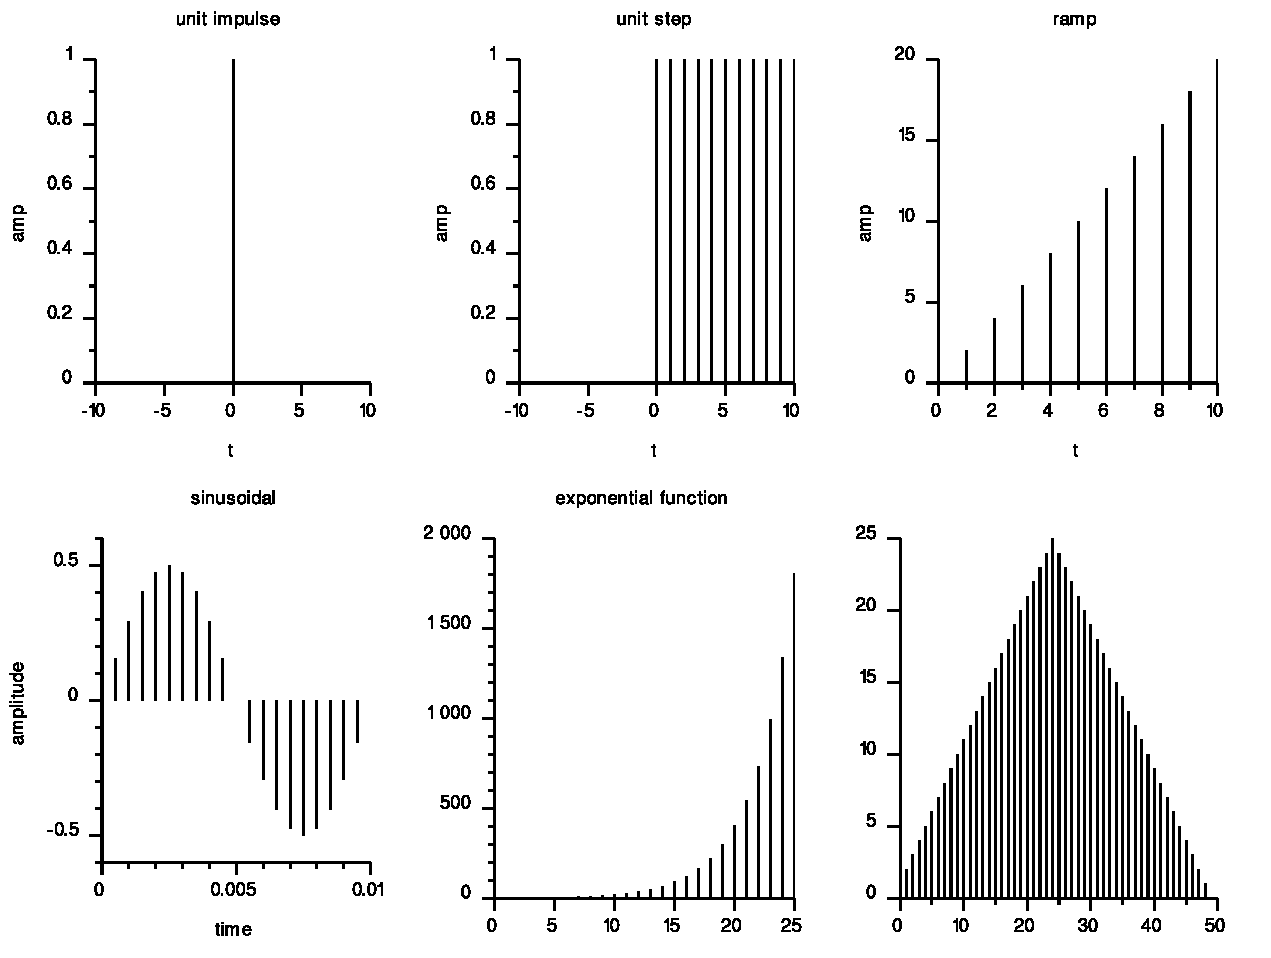
\includegraphics[scale=.5]{scilabCode/discrete.pdf}
\caption{Plot of discrete signals}
\label{discrete}
\end{figure}

\begin{figure}
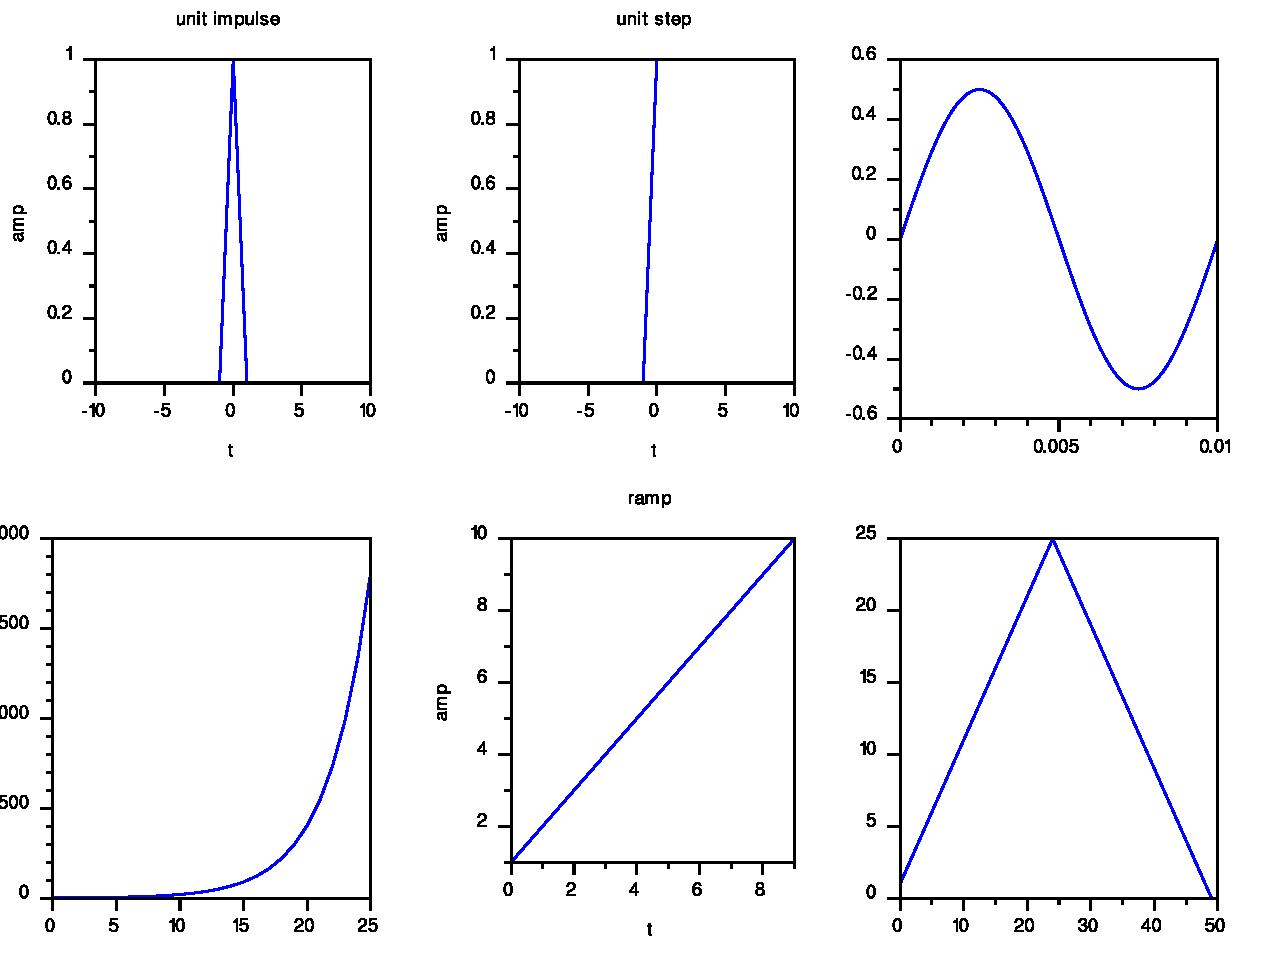
\includegraphics[scale=.5]{scilabCode/continuous.pdf}
\caption{Plot of continuous signals}
\label{continuous}
\end{figure}

\chapter [Solving Equations]{Solving Equations}


\section*{AIM}
\begin{itemize}
\item
To solve a linear equation in two variables accepting coefficients from the user.
\item 
To solve quadratic equation accespting coefficients from the user.

\end{itemize}

\section*{THEORY}
\paragraph{}

Linear equations can be solved using $linsolve()$ function.

\paragraph{}

\section*{PROCEDURE}

\paragraph{}
\begin{enumerate}
\item
Start Scilab on PC and Scilab console window opens. Create a new blank SciNote.
\item
The code for the required program is typed and saved as Scilab SCE file with an extension .sci
\item
The program is run using the “execute”.
\item
On executing the program in listing \ref{linEqn}, the following prompt appears on the Scilab console.

\begin{lstlisting}[numbers=none]
Enter the coefficients of first equation(Enter a1.x+b1.y=c1 as [a1 b1 -c1]:
\end{lstlisting}

For the equation $3x+2y=1$, input [3 2 -1] as shown below and press  `Enter'.
\begin{lstlisting}[numbers=none]
Enter the coefficients of first equation(Enter a1.x+b1.y=c1 as [a1 b1 -c1]:[3 2 -1] 
\end{lstlisting}
Enter the values of coeffiecients of second equation when prompted as
\begin{lstlisting}[numbers=none]
Enter the coefficients of second equation(Enter a2.x+b2.y=c2 as [a2 b2 -c2]:
\end{lstlisting}
For the equation $2x+4y=5$, input [2 4 -5] as shown below and press  `Enter'.
\begin{lstlisting}[numbers=none]
Enter the coefficients of second equation(Enter a2.x+b2.y=c2 as [a2 b2 -c2]:[2 4 -5]
\end{lstlisting}
\item
THe following prompt appears on the console on executing code in listing \ref{quadEqn}
\begin{lstlisting}[numbers=none]
Solving Quadratic Equations   
 
 ----------------------------   
 
     
Enter the coefficients(Eg: To solve c+(b*x)+a(x^2)=0, enter [c b a]):
\end{lstlisting}

For the equation $3+5x+6x^2=0$, input [3 5 6] and press `Enter'.
\item

The results and the errors in the program are displayed in the console window.
\end{enumerate}

\section*{SCILAB CODE}
\subsection*{Solve Linear equations in two variables}


\lstinputlisting[caption={Code to solve linear equation in two variables},label={linEqn}]{./scilabCode/LinearEquation.sci}

\subsection{Solve quadratic equation}

\lstinputlisting[caption={Code to solve quadratic equation},label={quadEqn}]{./scilabCode/quadEquation.sci}

\section*{RESULT}

For the program in listing \ref{linEqn} and the inputs as defined in procedure 4, following will be the final result.
\begin{lstlisting}[numbers=none]
The solutions are x=-0.750 and y=1.625
\end{lstlisting}



For the program in listing \ref{quadEqn} and the inputs as defined in procedure 4, following will be the final result.
\begin{lstlisting}[numbers=none]
1st root of the equation is =   
 
  - 0.4166667 + 0.5713046i  
 
 2nd root of the equation is   
 
  - 0.4166667 - 0.5713046i  
 
 The roots found using built in roots() function:   
 
  - 0.4166667 + 0.5713046i  
  - 0.4166667 - 0.5713046i
\end{lstlisting}



\chapter [Plotting the Diode characteristics]{Plotting the Diode characteristics}


\section*{Problem definition}

This experiment requires to plot the forward characteristics of a diode. 

\section*{Background Details}
\paragraph{}

The charcteristic equation that governs the current flow throgh a diode when it is forward biased is given by:

\begin{equation}
Id=Is\ exp(\frac{Vd}{n Vt}-1)
\end{equation}
\paragraph{}

\section*{Let us experiment}

\paragraph{}
\begin{enumerate}
\item
Start Scilab on PC and Scilab console window opens. Create a new blank SciNote.
\item
The code for the required program is typed and saved as Scilab SCE file with an extension .sci
\item
The program is run using the “execute”.
\item
On executing the program in listing \ref{linEqn}, the following graph appears on the figure window

\end{enumerate}


\section*{SCILAB Code}
\subsection*{Plotting the diode characteristics}


\lstinputlisting[caption={Code to plot the voltage current graph of a diode},label={diodeFBchar}]{./scilabCode/diodeFBchar.sci}


\section*{Plot and Results}

For the program in listing \ref{diodeFBchar} the following figure \ref{diodeFBcharFig} results.

\begin{figure}
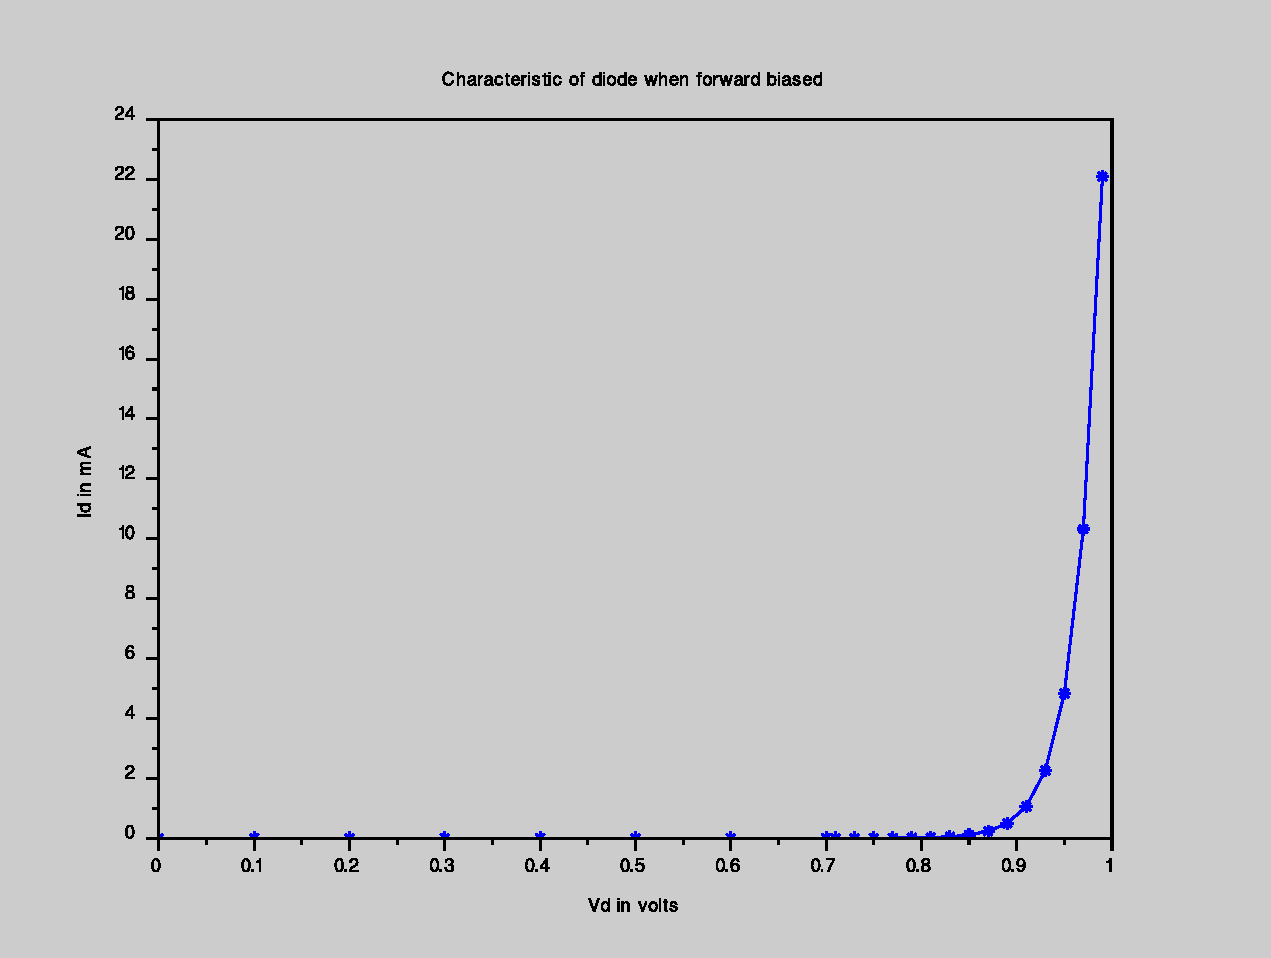
\includegraphics[width=\textwidth]{scilabCode/diodeFBchar.pdf}
\caption{Plot of Forward Characteristics of Diode}
\label{diodeFBcharFig}
\end{figure}




%\begin{appendix}
%\input{chapters/referencedata.tex}
%\end{appendix}
\begin{thebibliography}{1}

\bibitem{scilab}{\href{http://www.scilab.org/}{Scilab Official Website}}

\bibitem{spoken}{\href{http://scilab.in/spoken-tutorial}{Scilab Spoken Tutorial}}


\bibitem{tutorial}{\href{https://www.cse.iitb.ac.in/~cs626-449/scilab.pdf}{Scilab Tutorial}}

\end{thebibliography}


\end{document}
